\documentclass[tikz]{standalone}
\usepackage{pgfplots}
\pgfplotsset{compat=1.15}
\usepackage{mathrsfs}
\usetikzlibrary{arrows,calc}
\usepackage{tkz-euclide}
\pagestyle{empty}

\definecolor{AngleClr}{rgb}{0,0.39215686274509803,0}
\definecolor{ShapeClr}{rgb}{0.6,0.2,0}
\definecolor{BlueSqr}{RGB}{5,81,163}

\begin{document}

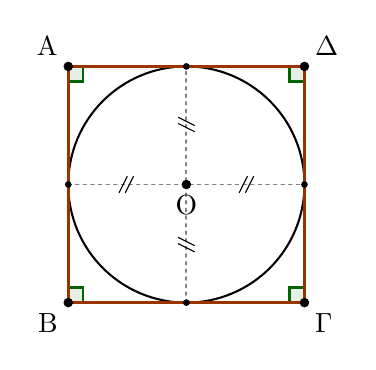
\begin{tikzpicture}[scale=.75]
\tkzSetUpLine[line width=1pt,color=black]
\tkzSetUpPoint[fill=black]

\tkzDefPoints{0/0/B,4/0/C,0/4/A,4/4/D}

\tkzDefMidPoint(A,C) \tkzGetPoint{O}
\tkzDefMidPoint(A,B) \tkzGetPoint{M1}
\tkzDefMidPoint(B,C) \tkzGetPoint{M2}
\tkzDefMidPoint(C,D) \tkzGetPoint{M3}
\tkzDefMidPoint(D,A) \tkzGetPoint{M4}

\tkzFillPolygon[fill=white](A,B,C,D)

\tkzMarkRightAngles[line width=1pt, size=.25,color=AngleClr,fill=AngleClr,fill opacity=0.1](A,B,C B,C,D C,D,A D,A,B)

\tkzDrawSegments[line width=0.7pt,color=gray,dashed,dash pattern=on 1pt off 1.75pt](M1,M3 M2,M4)
\tkzDrawCircle[line width=0.75pt,color=black](O,M1)

\tkzDrawPolygon[color=ShapeClr](A,B,C,D)
\tkzDrawPoints[size=3](A,B,C,D,O)
\tkzDrawPoints[size=2](M1,M2,M3,M4)
\tkzLabelPoint[above left](A){$\rm A$}
\tkzLabelPoint[below left](B){$\rm B$}
\tkzLabelPoint[below right](C){$\rm \Gamma$};
\tkzLabelPoint[above right](D){$\rm \Delta$};
\tkzLabelPoint[below](O){$\rm O$};

\tkzMarkSegments[mark=s||,size=3](O,M1 O,M2 O,M3 O,M4)


\end{tikzpicture}

\end{document}
